\section{MOS Stromquelle}
Bei der Einstellung des Arbeitspunkts mittels Widerstand resultiert eine quadratische Gleichung für den Strom und so die Ausgangsspannung eines Verstärkers.
Abhilfe kann eine Stromquelle anstelle des Widerstands schaffen.

MOS Transistoren sind bereits spannungsgesteuerte Stromquellen.
Durch einfügen eines $R_S$ kann der Innenwiderstand der Stromquelle \textbf{maximiert} werden. \textrightarrow\ Quelle wird 'idealer'

\subsection{Stromquelle -- Grundschaltungen}

% TODO: [Flurin] @ Simi: Schaltung mit R_S aus V6S18 und evtl. Formeln für R_iD aus V6S17
%CHECK: [Simi] @ Flurin: Falsche Slide für Schaltung im obigen todo..? Habe jetzt mal improvisiert...

\begin{minipage}[t]{0.44\columnwidth}
    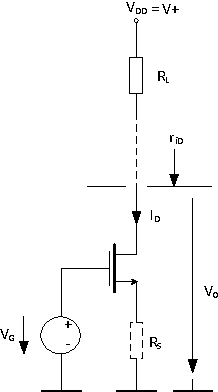
\includegraphics[width=0.48\columnwidth, align=t]{images/05_stromquelle_einfach_NMOS.pdf}
    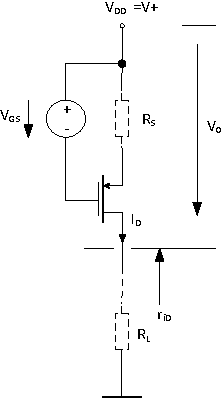
\includegraphics[width=0.48\columnwidth, align=t]{images/05_stromquelle_einfach_PMOS.pdf}
\end{minipage}
\hfill
\begin{minipage}[t]{0.5\columnwidth}
    \paragraph{Ausgangswiderstand}

    \vspace{-0.4cm}
    % \[
    %     r_{\rm iD} = r_{\rm DS} \left( 1 + g_m R_S + \frac{R_S}{r_{\rm DS}} \right) = r_{\rm DS} (1 + g_m R_S) + R_S 
    % \]

    \begin{align*}
         r_{\rm iD} &= r_{\rm DS} \left( 1 + g_m R_S + \frac{R_S}{r_{\rm DS}} \right) \\ 
                    &= r_{\rm DS} (1 + g_m R_S) + R_S
    \end{align*}
            

    \paragraph{Minimale Ausgangsspannung}

    \vspace{-0.2cm}

    \[
        V_{\rm out} = V_O > V_{O , \rm min} = R_S I_D + D_{\rm DS, sat}
    \]
\end{minipage}


\subsection{Kaskoden}
Damit für die Stromquelle kein Widerstand verwendet werden muss, kann ein weiterer Transistor verwendet werden. Diese Schaltung wird Kaskode genannt.

Dabei wird der maximale Ausgangsstrom jedoch leicht reduziert.


\subsubsection{Kaskode -- Grundschaltung}
\label{Kaskode -- Grundschaltung}

\begin{minipage}[t]{0.3\columnwidth}
    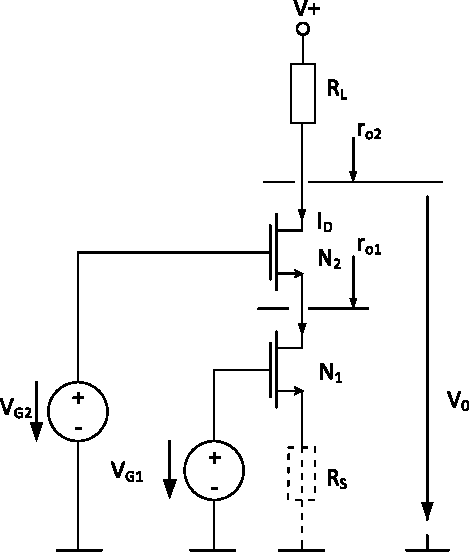
\includegraphics[width=\columnwidth, align=t]{images/05_stromquelle_kaskode.pdf}
\end{minipage}
\hfill
\begin{minipage}[t]{0.62\columnwidth}
    \paragraph{Ausgangswiderstand}

    \vspace{-0.2cm}
    \[
        r_{\rm out} = r_{\rm o2} \approx g_{m2} \cdot r_{\rm DS}^2 = a_{\rm max} \cdot r_{\rm DS}
    \]
            

    \paragraph{Minimale Ausgangsspannung}

    \vspace{-0.5cm}
    \[
        V_{O, \rm min} = V_{\rm G2} - V_{\rm GS2} + V_{\rm DS2, sat} =  V_{\rm DS1, sat} + V_{\rm DS2, sat}
    \]


    \paragraph{Strom}

    \vspace{-0.4cm}
    \[
        I_D = \frac{\mu C_{\rm ox}}{2} \left( \frac{W}{L}\right)_{N1} (V_{\rm GS\_N1} - V_T)^2 \cdot \cbl{(1 + \lambda V_{\rm DS\_N1})}
    \]
\end{minipage}


\subsubsection{Geregelte Kaskode}
Um die Kaskodenschaltung weiter zu \textbf{verbessern}, kann die $V_\text{GS}$ Spannung des oberen Transistors auf die Referenzspannung geregelt werden.
Durch das Stabilisieren der Spannung wird der Arbeitspunkt des Transistors stabilisiert (indem $I_D$ konstant ist) und der \textbf{Ausgangswiderstand noch grösser}.

\smallskip

\begin{minipage}[t]{0.55\columnwidth}
    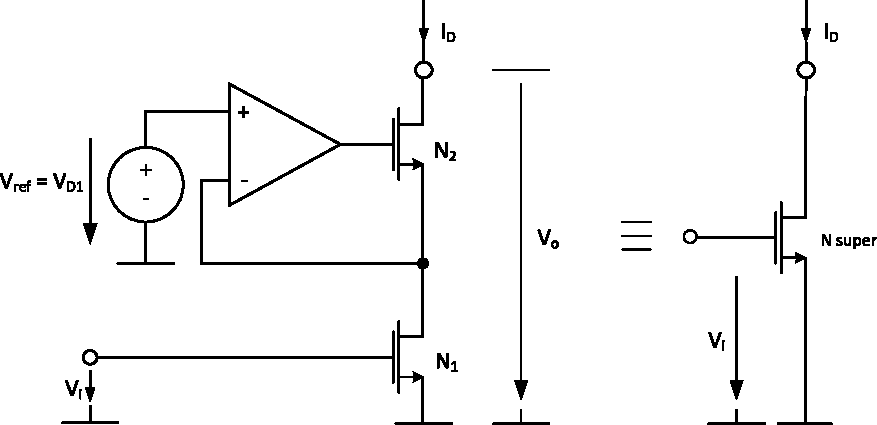
\includegraphics[width=\columnwidth, align=t]{images/05_stromquelle_geregelte_kaskode_opamp.pdf}
\end{minipage}
\hfill
\begin{minipage}[t]{0.42\columnwidth}

    \paragraph{Transkonduktanz}

    \vspace{-0.3cm}
    \[
        g_{m,\rm super} = g_{m1}
    \]            

    \paragraph{Minimale Ausgangsspannung}

    \vspace{-0.2cm}
    \[
        V_{O, \rm min} =  V_{\rm ref} + V_{\rm DS2, sat}
    \]

    \paragraph{Strom}

    \textrightarrow\ Siehe Grundschaltung (\ref{Kaskode -- Grundschaltung})
\end{minipage}


\paragraph{Ausgangswiderstand}

\vspace{-0.3cm}
\[
    r_{\rm out} \approx r_{\rm DS1} \cdot g_{m2} \cdot r_{\rm DS2} \cdot (a + 1) = \frac{1}{g_{o1}} \cdot \frac{g_{m2}}{g_{o2}} \cdot (a + 1)
\]


\subsubsection{Säckinger Kaskode}
Die Säckinger Kaskode ersetzt den komplexen OpAmp mit einem einzelnen Transistor ($\rm N_3$) in \textbf{Source-Schaltung}.

\smallskip

\begin{minipage}[t]{0.55\columnwidth}
    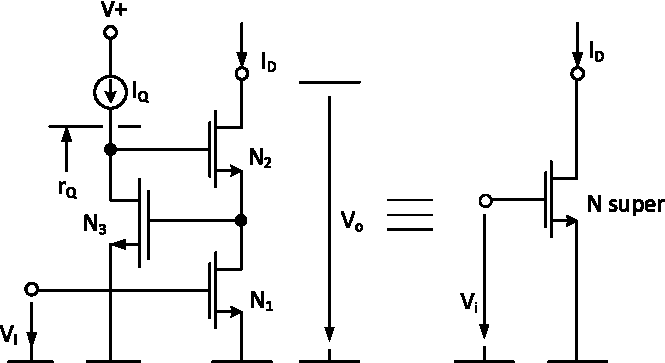
\includegraphics[width=\columnwidth, align=t]{images/05_stromquelle_geregelte_kaskode_FET.pdf}
\end{minipage}
\hfill
\begin{minipage}[t]{0.42\columnwidth}

    \paragraph{Transkonduktanz}

    \vspace{-0.3cm}
    \[
        g_{m,\rm super} = g_{m1}
    \]            

    \paragraph{Minimale Ausgangsspannung}

    \vspace{-0.2cm}
    \[
        V_{O, \rm min} =  V_{\rm GS3} + V_{\rm DS2, sat}
    \]

    \paragraph{Strom}

    \textrightarrow\ Siehe Grundschaltung (\ref{Kaskode -- Grundschaltung})
\end{minipage}


\paragraph{Ausgangswiderstand}

\vspace{-0.3cm}
\[
    r_{\rm out} \approx r_{\rm DS1} \cdot g_{m2} r_{\rm DS2} \cdot g_{m3} r_{\rm DS3} = \frac{1}{g_{o1}} \cdot \frac{g_{m2}}{g_{o2}} \cdot \frac{g_{m3}}{g_{o3}}
\]

